\parindent=0em
\section{Pruebas de geolocalización sobre ARCore}
\label{pruebas geo arcore}
\noindent

Una vez obtenido el archivo \textit{.json} con toda la información de la ruta como se ha comentado en el punto~\ref{mapboxbusquedarutas}, el siguiente paso fue crear una aplicación que utilizase dicha información.\\

El objetivo principal de la aplicación era transformar coordenadas de latitud y longitud a una posición en el entorno de ARCore.\\

Para ello, se integró ARCore en un proyecto de Unity como se ha contado en el punto~\ref{integracionARCOREUNITY} y además, se agregó un \textit{package} que facilita la página oficial de Mapbox para ser incluido en Unity. Una vez agregado el paquete de creó una \textit{API Key} (identificador único para autenticar a un usuario al hacer una llamada a una API) en Mapbox y se añadió al archivo de propiedades de Mapbox en Unity (para poder utilizar sus distintos servicios).\\

Teniendo un proyecto en Unity con Mapbox y ARCore integrados el siguiente paso fue transformar las coordenadas de latitud y longitud a un punto de ARCore. Primero de todo se obtuvo la latitud y longitud del dispositivo a través de la señal del GPS.\\

A continuación, se transformó esas coordenadas a un punto en el mundo de Unity. Para ello se aplican las siguientes fórmulas de cara a convertir latitud y longitud a metros en el eje \textbf{\textit{x}} y el eje \textbf{\textit{y}} de Unity. Posteriormente, estos valores en metros se transforman para un mapa con una escala de 2.5 metros por 1 unidad de Unity quedando ajustados así a la posición respectiva según la latitud y longitud.\\


%https://docs.mapbox.com/mapbox-unity-sdk/api/unity/Mapbox.Unity.Utilities.Conversions.html#Mapbox_Unity_Utilities_Conversions_GeoToWorldPosition_System_Double_System_Double_Vector2d_System_Single_

En primer lugar es necesario conocer la constante \textit{OriginShift} que se obtiene con la siguiente fórmula (teniendo en cuenta un valor del radio de la tierra de 6.378.137):\\

\[OriginShift = \frac{2\pi\cdot EarthRadius}{2}\]\\

Por una parte la posición en el eje \textit{x} es calculada como:\\

\[x = \frac{longitud\cdot OriginShift}{180}\]\\

En cambio, el valor de la posición en el eje \textit{y} se obtiene a través de la fórmula:\\

\[y = \frac{\log(\tan\frac{(90+latitud)\cdot\pi}{360})}{\frac{\pi}{180}}\]\\

Una vez que se ha aplicado la fórmula anterior, para ajustar la posición \textit{y} respecto al origen igual que se ha hecho con la posición x se realiza el calculo de:\\

\[y = \frac{y \cdot OriginShift}{180}\]\\

Dado que la posición del objeto no solo se define en el eje \textit{x} e \textit{y}, sino que también hay que tener en cuenta el eje \textit{z}, se utiliza como posición un vector \textbf{targetPos} del siguiente modo:\\

\[\textbf{targetPos} = (x,0,y)\]\\

El vector \textbf{targetPos} es la correspondencia de la transformación de unas coordenadas de latitud y longitud al mundo de Unity. Para comprobar la precisión de la aplicación se realizaron dos pruebas distintas, una en interiores y otra en exteriores. Ambas pruebas se han realizado utilizando únicamente la señal GPS del teléfono móvil.\\

En primer lugar, se comprobó que en la aplicación en interiores se colocaba el elemento virtual cercano a las coordenadas como se puede ver en la figura~\ref{fig:mapboxinteriores} . Sin embargo, dicho posicionamiento de los elementos virtuales (en este caso un cubo de color gris) tenía una desviación en las coordenadas de entre 1 y 2 metros.

\begin{figure}[H]
\centering
    \hspace{-4mm}
    \begin{minipage}{0.5\textwidth}
        \centering
        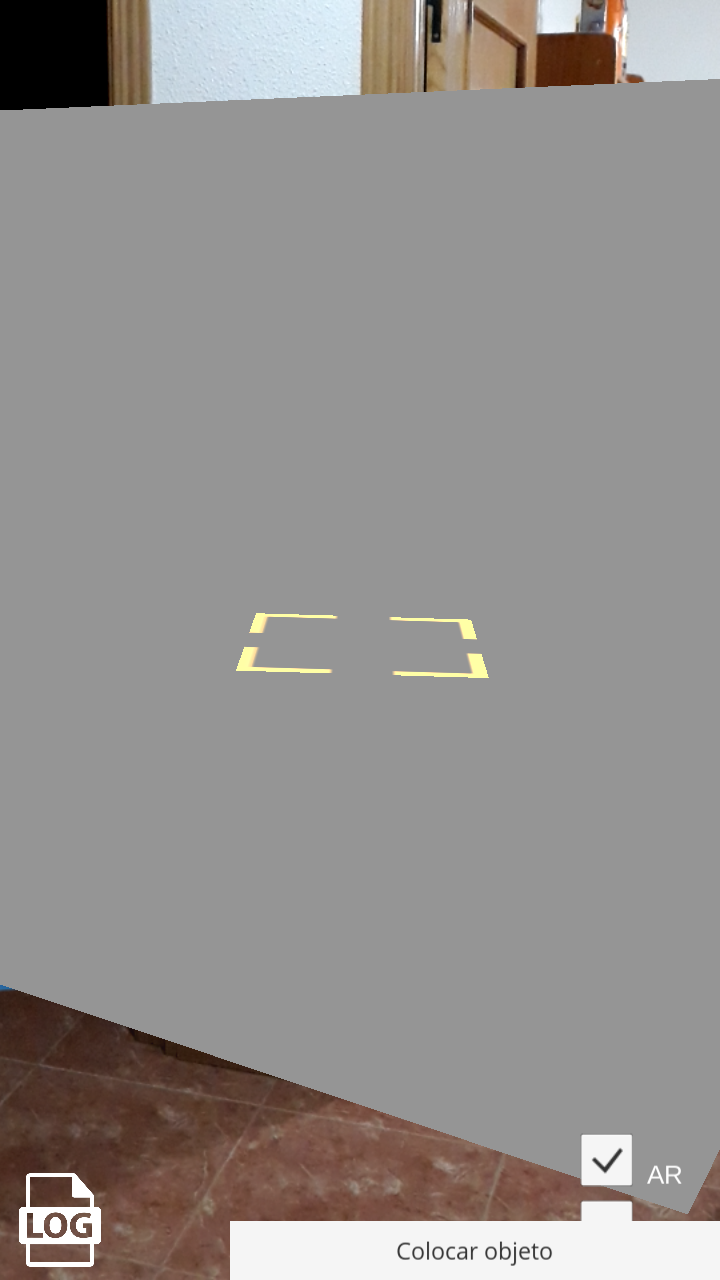
\includegraphics[scale=0.25]{Images/PruebasMapbox/mapboxGPS (1).png}\\
    \end{minipage}
    \begin{minipage}{0.5\textwidth}
        \centering
        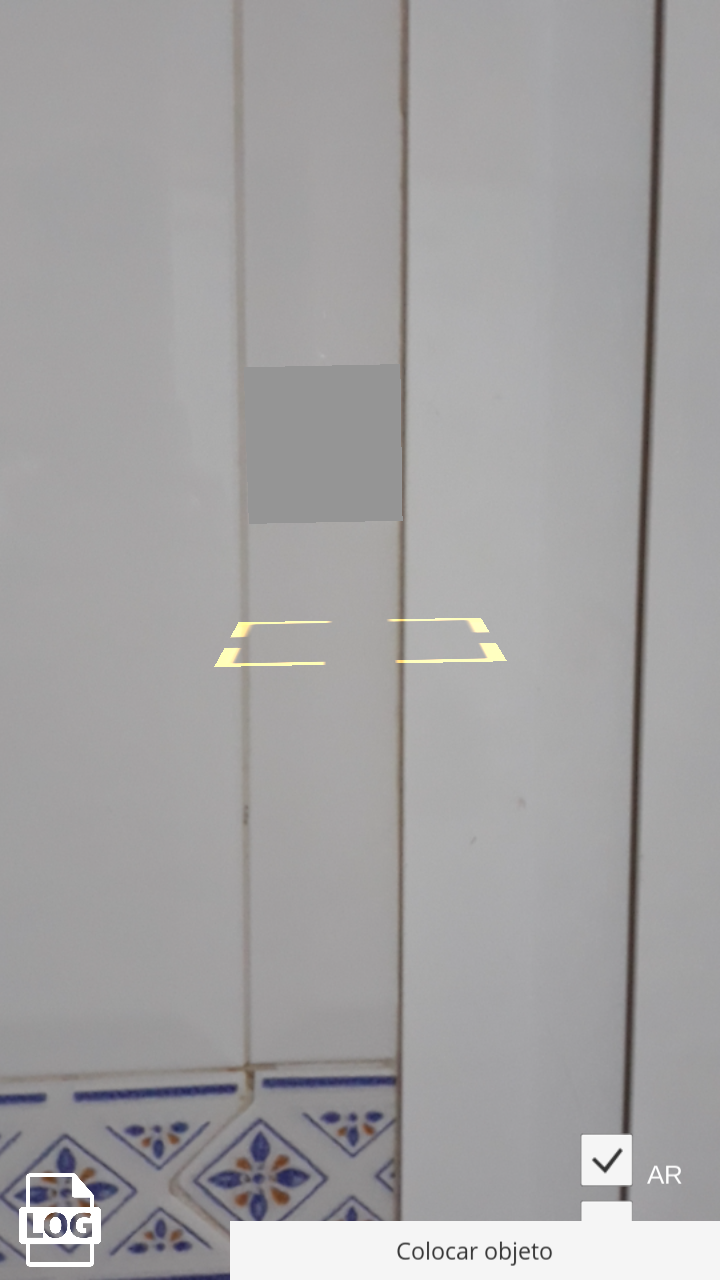
\includegraphics[scale=0.25]{Images/PruebasMapbox/mapboxGPS (6).png}\\
    \end{minipage}\\
    \caption{Pruebas de la transformación de coordenadas en interiores.}
    \label{fig:mapboxinteriores}
\end{figure}


Dado que las coordenadas en exteriores suelen ser más precisas, se pasó a probar el funcionamiento de la aplicación en exteriores. El resultado obtenido fue muy similar al resultado en interiores como se aprecia en la figura~\ref{fig:mapboxexteriores}.\\


Se estima que utilizando un teléfono con cobertura móvil, se podría reducir el error del modo que la desviación sería de entre 0,5 y 1 metros. Esta nueva desviación se obtendría gracias al A-GPS.

\begin{figure}[H]
\centering
    \hspace{-4mm}
    \begin{minipage}{0.5\textwidth}
        \centering
        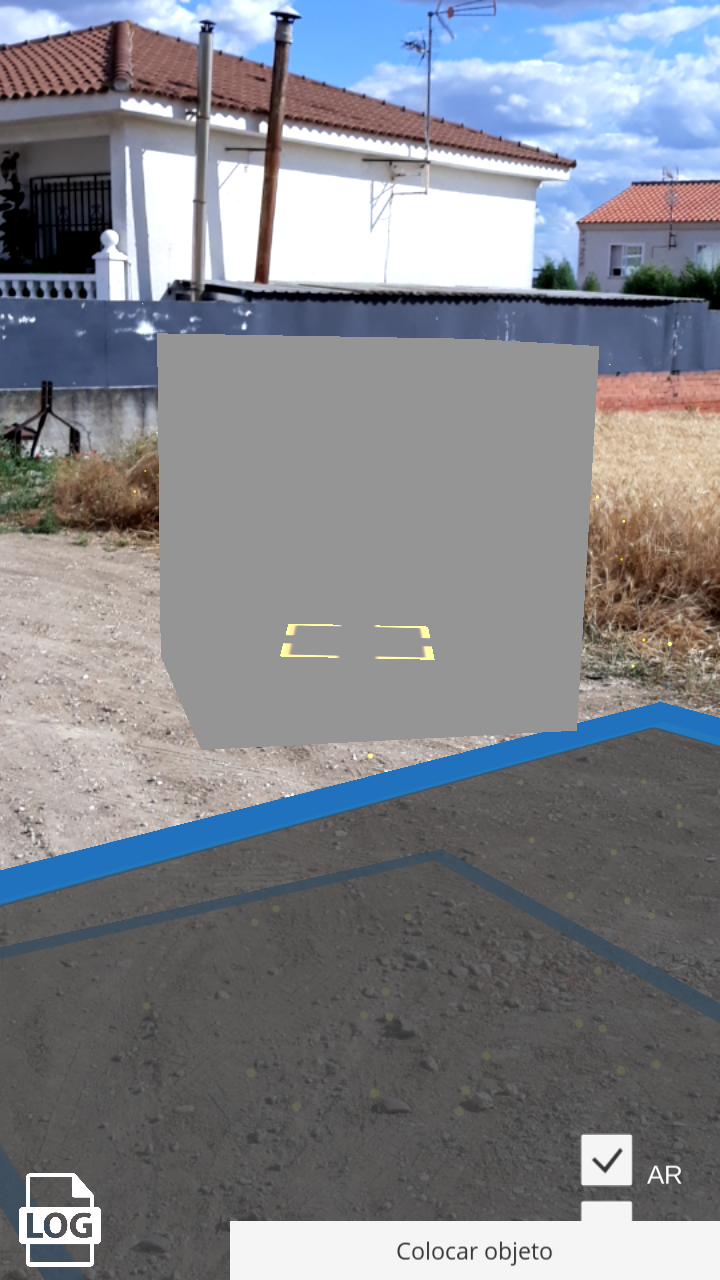
\includegraphics[scale=0.25]{Images/PruebasMapbox/mapboxGPS (2).png}\\
    \end{minipage}
    \begin{minipage}{0.5\textwidth}
        \centering
        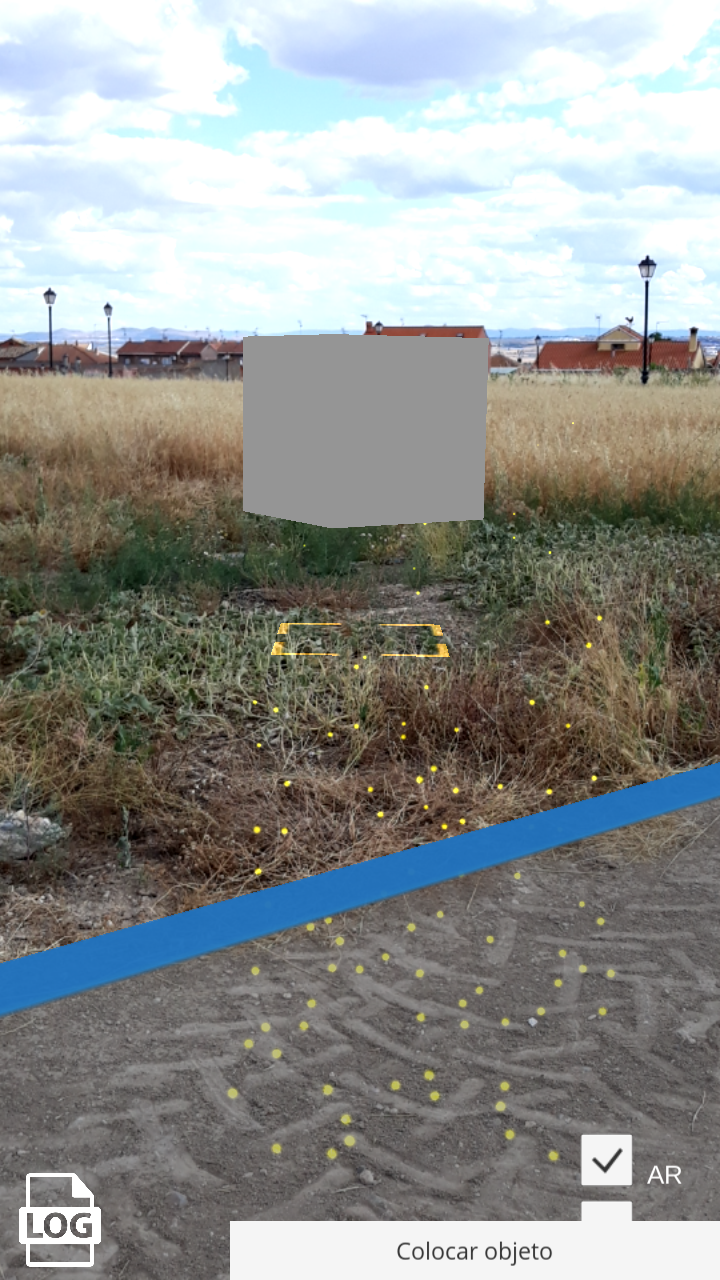
\includegraphics[scale=0.25]{Images/PruebasMapbox/mapboxGPS (4).png}\\
    \end{minipage}\\
    \caption{Pruebas de la transformación de coordenadas en exteriores.}
    \label{fig:mapboxexteriores}
\end{figure}

Como se puede observar, no existen grandes cambios en las pruebas en exteriores respecto a las pruebas en interiores. Se llegó a la conclusión de que esto se debe a utilizar únicamente la información del GPS y no tener la triangulación de las torres de telefonía que aportaría el A-GPS.

 












